%! TEX root = **/010-main.tex
% vim: spell spelllang=en:

\section{Context and scope}%
\label{sec:context}

\subsection{Introduction and contextualization}%
\label{sub:intro}

Since its release in 2007, Compute Unified Device Architecture (CUDA) has
revolutionized the usage of graphic processing units for scientific
computations, allowing developers to implement programs that take full advantage
of the parallelization capabilities of Graphics Processing Units (GPUs) for
general purpose programming. This paired with the exponential growth of
computing power that GPUs have experienced in the last decade has made GPU
numerical analysis essential in modern science research. Highly complex problems
that were once impossible to compute in realistic time frames can now be
computed even on average consumer hardware GPUs. Moreover, projects like
\emph{GPUGRID}\footnote{\url{www.gpugrid.net}} allow researchers to run
distributed programs through a grid of GPUs from volunteers all over the world
reaching supercomputing level performance \cite{antaviana_nvidia_2008}.

In 1900 David Hilbert posed a list of 23 important problems in the field of mathematics
which were unsolved at the time
\cite{hilbert_mathematische_1900,hilbert_mathematical_1902}. Those
problems have been vastly studied since then and most of them are solved or
partially solved. There are however some which are still unsolved to this day.

One of the still unsolved problems is the 16th problem. This problem consists of
two separate problems, the first one regarding the relative positions of the
branches of real algebraic curves and the second one about the upper limit of
{\em limit cycles} on two-dimensional vector fields and their relative positions. In
this project we are going to study the second part of this 16th problem.

In particular, we study the number of limit cycles for vector fields of
polynomials of second degree:
\begin{align}\label{eq:system}
    \frac{dx}{dt} &= a_1x^2 + b_1xy + c_1y^2 + \alpha_1x + \beta_1y \nonumber \\
    \frac{dy}{dt} &= a_2x^2 + b_2xy + c_2y^2 + \alpha_2x + \beta_2y
\end{align}

Solving the system of differential equations~(\ref{eq:system}) results in a trajectory $x(t), y(t)$ which represents some curve on $(x, y)$ plane. There are different possibilities for how this curve looks like. One of the most interesting cases is when it results in an {\it attractor}. An attractor is defined as a compact subset of the phase space of a dynamical system, such that all trajectories from some neighborhood of it tend to it at infinite time. An attractor can be an attracting fixed point or as well a periodic trajectory (limit cycle).

\begin{itemize}
\item the trajectory goes away to infinity
\item the trajectory goes to a fixed point
\item the trajectory goes to a limit cycle
\end{itemize}

It is unknown whether there exists an upper limit on the number of limit cycles
for systems with polynomials of degree greater than
one~\cite{christopher_hilberts_2007,ilyashenko_centennial_2002,llibre_sobre_2015}.
Nowadays, the largest number of limit cycles found is equal to four. It is
still an open question whether or not a larger number of limit cycles is
possible. Therefore, finding a system with 4 limit cycles or more will be quite
an important result for the academic community.

%???
%
%Do I remove this?
%
% To find interesting systems several combinations of the equation parameters
% must be tried and evaluated, since each of these systems can be computed
% independently of the rest they can all be run in parallel, making it an ideal
% problem to compute in massively parallel GPU nodes.

\subsubsection{Context}

This is a Bachelor Thesis of the Computer Engineering Degree, specialization in
Computing, done in the \textcatalan{Facultat Inform\`atica de Barcelona (FIB)}
of the \textcatalan{Universitat Polit\'ecnica de Catalunya (UPC)}. The project
is directed by Grigori Astrakharchik.

\pagebreak
\subsubsection{Concepts}

Below are some concepts needed to understand the project.

\paragraph{Limit cycles}

A limit cycle is a closed trajectory with the property that at least one other
trajectory spirals into it as time approaches infinity. They are important in
various applications in the field of dynamical systems.

\paragraph{CUDA}
CUDA is a parallel computing platform developed by \emph{nvidia} that allows general
computing on their graphic processing units (GPUs). Using the CUDA programming
model allows developers to run massively parallel programs on GPUs.

\pagebreak
\subsubsection{Problem to be solved}

There have been various studies on the number of limit cycles for second degree
vector fields but so far the maximum number of cycles found is 4, as reported in
Ref.~\cite{kuznetsov_visualization_2013}. The aim of this project is to search
the parameter space for systems that have 4 or more cycles to gain more insight
on the nature of these equations.

\Cref{fig:kuznetsov} shows a characteristic example of a visualization of the
limit cycles in a two-dimensional polynomial quadratic system.

\begin{figure}[H]
    \centering
    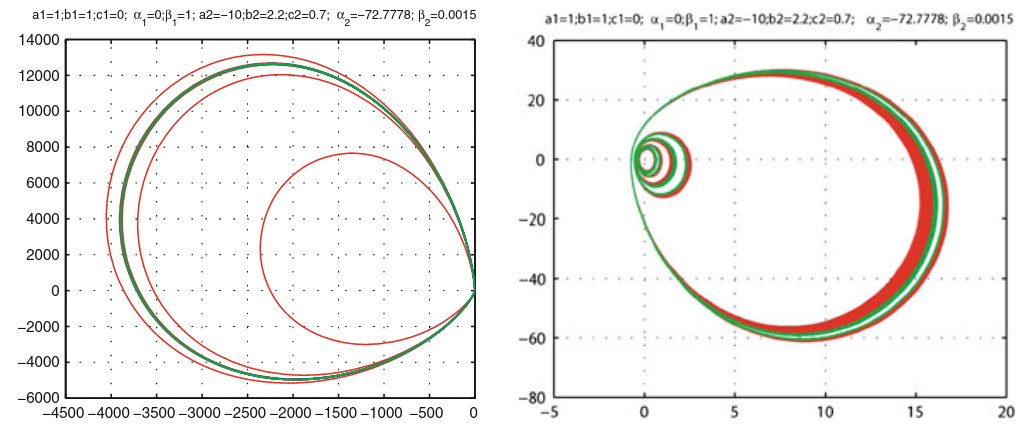
\includegraphics[width=1.0\textwidth]{4cycles}
    \caption{Visualization of four limit cycles in two-dimensional polynomial quadratic system, from Ref.~\cite{kuznetsov_visualization_2013}
    }%
    \label{fig:kuznetsov}
\end{figure}

We implement an efficient parallel algorithm that solves systems of ordinary differential equations (ODE) and detects limit cycles for a wide range of parameters and points in the plane. This code is implemented in Julia programming language and will use CUDA framework in such a way that massive parallel calculation can be done on a dedicated CUDA server with several
advanced GPU graphic cards.

\pagebreak

\subsection{Computational complexity}

The system of differential equations~\cref{eq:system} contains 5 free coefficients for $x$ and 5 more for $y$ which makes a total of 10 distinct parameters. Adding the initial point to calculate the trajectories ($x$ and $y$ coordinates) it makes a total of 12 free parameters. Thus, the total space of parameters to be investigated is huge. Fortunately, the number of coefficients in the study can be reduced further to only 5 independent ones (parameters for $x$ are 1) as given in~\cref{eq:system2}.
\begin{align}\label{eq:system2}
    \frac{dx}{dt} &= x^2 + xy + y^2 + x + y \nonumber \\
    \frac{dy}{dt} &= a_2x^2 + b_2xy + c_2y^2 + \alpha_2x + \beta_2y
\end{align}
This ends up in a total of 7 independent parameters.

If we consider $n$ different values for each of those parameters we have a total of $n^7$ different trajectories to calculate. For example, for $n=100$ different values for each parameter, $10^{14}$ trajectories has to be calculated in order to sample the space of available parameters. If we were to compute the trajectories sequentially it would take an exceedingly long time even for moderately sized values of $n$. Calculating a trajectory on a typical desktop machine takes 0.01 seconds. This means that for $n=10$ it would take approximately 28 hours to compute all the trajectories and taking $n=30$ the time increases to 7 years. If we were to use a GPU with 5000 CUDA cores (Tesla K90) it would only take 20 seconds (assuming perfect parallelization). And for $n=30$ it would take 12 and a half hours. Thus, the use of CUDA clusters, like Minotauro in Barcelona Supercomputing Center, looks very promising. If we consider the usage of a cluster composed of 39 servers with 2 Tesla K90 GPUs the computation time for $n=30$ is estimated to be a mere 9 minutes. \footnote{All these calculations are based on a very rough estimate of the computing time needed to determine the limit cycle of a trajectory which may vary a lot depending on the system and the implementation of the code}

\subsubsection{Stakeholders}

The main stakeholders in this project are the researcher (me) and the director,
Grigori Astrakharchik, that have a direct implication on the Thesis. If we manage
to obtain interesting results other parties may benefit from them: other
researchers on the fields of numerical analysis and dynamic systems may build on
these results.

\pagebreak
\subsection{Justification}

In~\cite{kuznetsov_visualization_2013} there is a description of a task given by
the academician A.N.~Kolmogorov:

\begin{quote}
To estimate the number of limit cycles of square vector fields on plane, A.N.~Kolmogorov had distributed several hundreds of initial parameters (with randomly chosen coefficients of quadratic expressions) among a few hundreds of students of Mech \& Math Faculty of Moscow State University as a mathematical practice. Each student had to find the number of limit cycles of a field. The result of this experiment was absolutely unexpected: not a single field had a limit cycle!
\end{quote}

This shows that the parallelizable nature of the problem and how difficult it is to find those cycles. Therefore, it is important to implement a code that is both efficient on the calculation and have a big enough search space to find results.
% {\bf In particular, in examples studied in this Thesis, the number of studied trajectories is $10^8$ ??? Which far more as compared to $10^2$ as performed by Kolmogorov with his students.}

\subsubsection{Previous studies}

There has been a number of studies relying on numerical methods to find limit cycles in two-dimensional vector fields
\cite{leonov_hidden_2013,van_der_hoff_numerical_2013,casades_computation_2013,gasull_effective_2015}.
Papadimitriou and Vishnoi showed that the computation of a limit cycle is
PSPACE-complete~\cite{papadimitriou_computational_2015}.
The maximal known number of limit cycles is reported in Kuznetsov et al.~\cite{kuznetsov_visualization_2013} where an example of specific conditions for which \textbf{4 limit cycles} is provided.

All the previous studies have relied on standard analytical methods to calculate trajectories and find limit cycles, there has not been research on developing efficient parallel code to solve ODE trajectories on GPUs with the aim of finding limit cycles. This projects aims to develop a highly efficient method to aid the search of limit cycles using modern computational capabilities. At best, we will be able to find systems with 4 or more limit cycles on our search, at worst the developed code will still be useful to quickly analyze systems in search of limit cycles.

\pagebreak
\subsubsection{CUDA and Julia}

The CUDA framework has API for several programming languages (C, C++, Fortran,
Python, MATLAB, \dots). The official programming toolkit~\cite{nvidia_cuda_2021}
is in C/C++ and offers the most customizability and low level configuration to
adapt the code to the hardware. The two most notable alternatives are Python's
\emph{pyCUDA}~\cite{klockner_pycuda_2012} and Julia's
\emph{CUDA.jl}~\cite{besard_effective_2019} libraries. These libraries bind to
the C CUDA API and interface the data between the kernels and the programming
language. As such, the performance of the kernels that run in the GPU should be
equivalent in all cases but the data models and processing of different
languages makes a difference when interfacing between the GPU code and the CPU
code.

However, languages such as Python and Julia allow for faster development of the
code and easier visualization of the data. For this Thesis we will use Julia
programming language since it's faster than Python, has many libraries and tools
for numerical analysis and has type checking. The performance of Julia CUDA
library has a 0.50\% impact on performance compared to C according to the
literature~\cite{besard_effective_2019}. Moreover, the
\emph{DifferentialEquations.jl} Julia
library~\cite{rackauckas_differentialequationsjl_2017} has been shown to
outperform C implementations of ODE solvers and currently is the most feature
complete and efficient suite for differential equation
solving~\cite{rackauckas_comparison_2017}.

\pagebreak
\subsection{Scope}
\subsubsection{Objectives and sub-objectives}

The main objective of this Thesis is to develop a highly-efficient code capable of determining the possible existence of limit cycles for a system. This code must also be capable of being executed in parallel in a GPU cluster making full use of its computing power to simulate a wide variety of systems with different parameters. Furthermore, the results must be processed to find interesting systems to visualize and analyze in more detail. These objectives can be divided in sub-objectives:

\paragraph{Theoretical part}

Before implementing the algorithms and developing the code, a deep understanding
of the current numerical methods and the CUDA framework must be achieved to find
the best approach to the problem.

\begin{itemize}
    \item Explore the best strategies to solve ordinary differential equations.
    \item Explore numerical methods to verify the existence of limit cycles and determine the number of cycles for a given system.
    \item Research how these methods can be applied to run in a CUDA system efficiently.
\end{itemize}

\paragraph{Practical part}

Having done the background research, the code must be developed, implemented and
tested.  Different methods will be tried in order to find the ones that give the
best performance.

\begin{itemize}
    \item Implement the algorithms in an efficient code.
    \item Benchmark the performance and compare different approaches to achieve the best performance.
    \item Run the code on a dedicated GPU server.
    \item Analyze the results and visualize them.
    \item Present and discuss the obtained results in the Thesis.
\end{itemize}

\subsubsection{Requirements}

To ensure the quality of the Thesis a number of requirements must be fulfilled:
\begin{itemize}
    \item Find the best balance between accuracy of the results and computational complexity
    \item Ensure that the numerical methods applied are properly implemented.
    \item Take into account numerical stability of the methods used as well as rounding and overflow errors.
    \item Profile the different methods under the same conditions and environment to ensure that there are no biases.
    \item Use good programming practices, making readable and maintainable code with the least complexity possible.
    \item Make the developed code publicly available.
\end{itemize}

\subsubsection{Potential obstacles and risks}%
\label{ssub:intro_risks}

There are several risks that may have to be dealt with during the development of this Thesis.

\begin{itemize}
    \item \textbf{Project deadlines}: There is a limited amount of time to do
        the project. Therefore, a proper planning of tasks and time must be made
        and followed to ensure that the work can be done in the proper time
        frame.
    \item \textbf{Computational power}: This Thesis involves a lot of
        computational power and the whole project is conditioned by it. If the
        program cannot be run on the proper hardware the results may not be
        obtainable in a realistic time frame and the scope of the project will
        have to be reevaluated.
    \item \textbf{Inexperience on the field}: I have very limited experience
        with CUDA programming and just the basics of numerical computation
        techniques, so there is a lot of research to be done, specially regarding
        dynamical systems.
\end{itemize}

\pagebreak
\subsection{Methodology and rigor}

\subsubsection{Methodology}

Since the Thesis must be completed in a relatively short period of time we will
apply the \emph{agile} methodology and divide the work into sub-tasks or
\emph{sprints}. These \emph{sprints} will consist of different stages of
implementation of the program, beginning with a proof of concept running in
sequence on the CPU and progressively iterating on this base to optimize the
methods and adapt them to be able to run in CUDA on the GPU.

\subsubsection{Monitoring tools and validation}

To manage the different iterations of the code \texttt{git} will be used,
this will allow to have a complete history of the different changes to the code
made during the project. Different branches will be used during the development
of the code: a \emph{master} branch with the current working code, a
\emph{development} branch in which the newest features are added. When the work done
in the \emph{development} branch is properly tested and proved to be working the
changes will merge into the \emph{master} branch. Additionally, some
other branches may be created with experimental changes.

The \texttt{git} repository will be hosted on \href{github.com}{GitHub} and
access will be granted to the project tutor allowing him to follow and monitor
the work and results at any time. To control the bugs and features added to the
code \emph{GitHub}'s issue system will be used, this issues will be classified
with labels and managed through \emph{GitHub}'s project system (using kanban style
project boards) following \emph{GitHub}'s guidelines on project management with
their platform~\cite{github_managing_2021}.  Every time a milestone is reached a
new signed label will be added to the repository to keep track of the most
relevant points in the development of the program. The repository will be
private during the development of the thesis but will be made publicly available
to the community once it's finished.

The thesis' document will also be tracked with \texttt{git} and hosted on
\emph{GitHub} similarly to how the code is monitored. However, the document
repository will also be synced to \href{overleaf.com}{Overleaf} allowing online
edition of the document.

A weekly meeting with the tutor will be arranged to discuss the progress and
which tasks should be worked on.
